


\newpage
\addcontentsline{toc}{section}{Design Flow}
\section*{ \hfill Design Flow}

% \lipsum

\addcontentsline{toc}{subsection}{IP Customization and Generation }
\subsection*{\fontsize{14}{16}\selectfont IP Customization and Generation}
OCLA IP core is a part of the Raptor Design Suite Software. A customized ocla can be generated from the Raptor's IP configurator window.
\begin{figure}[h]\centering % Using \begin{figure*} makes the figure take up the entire width of the page
	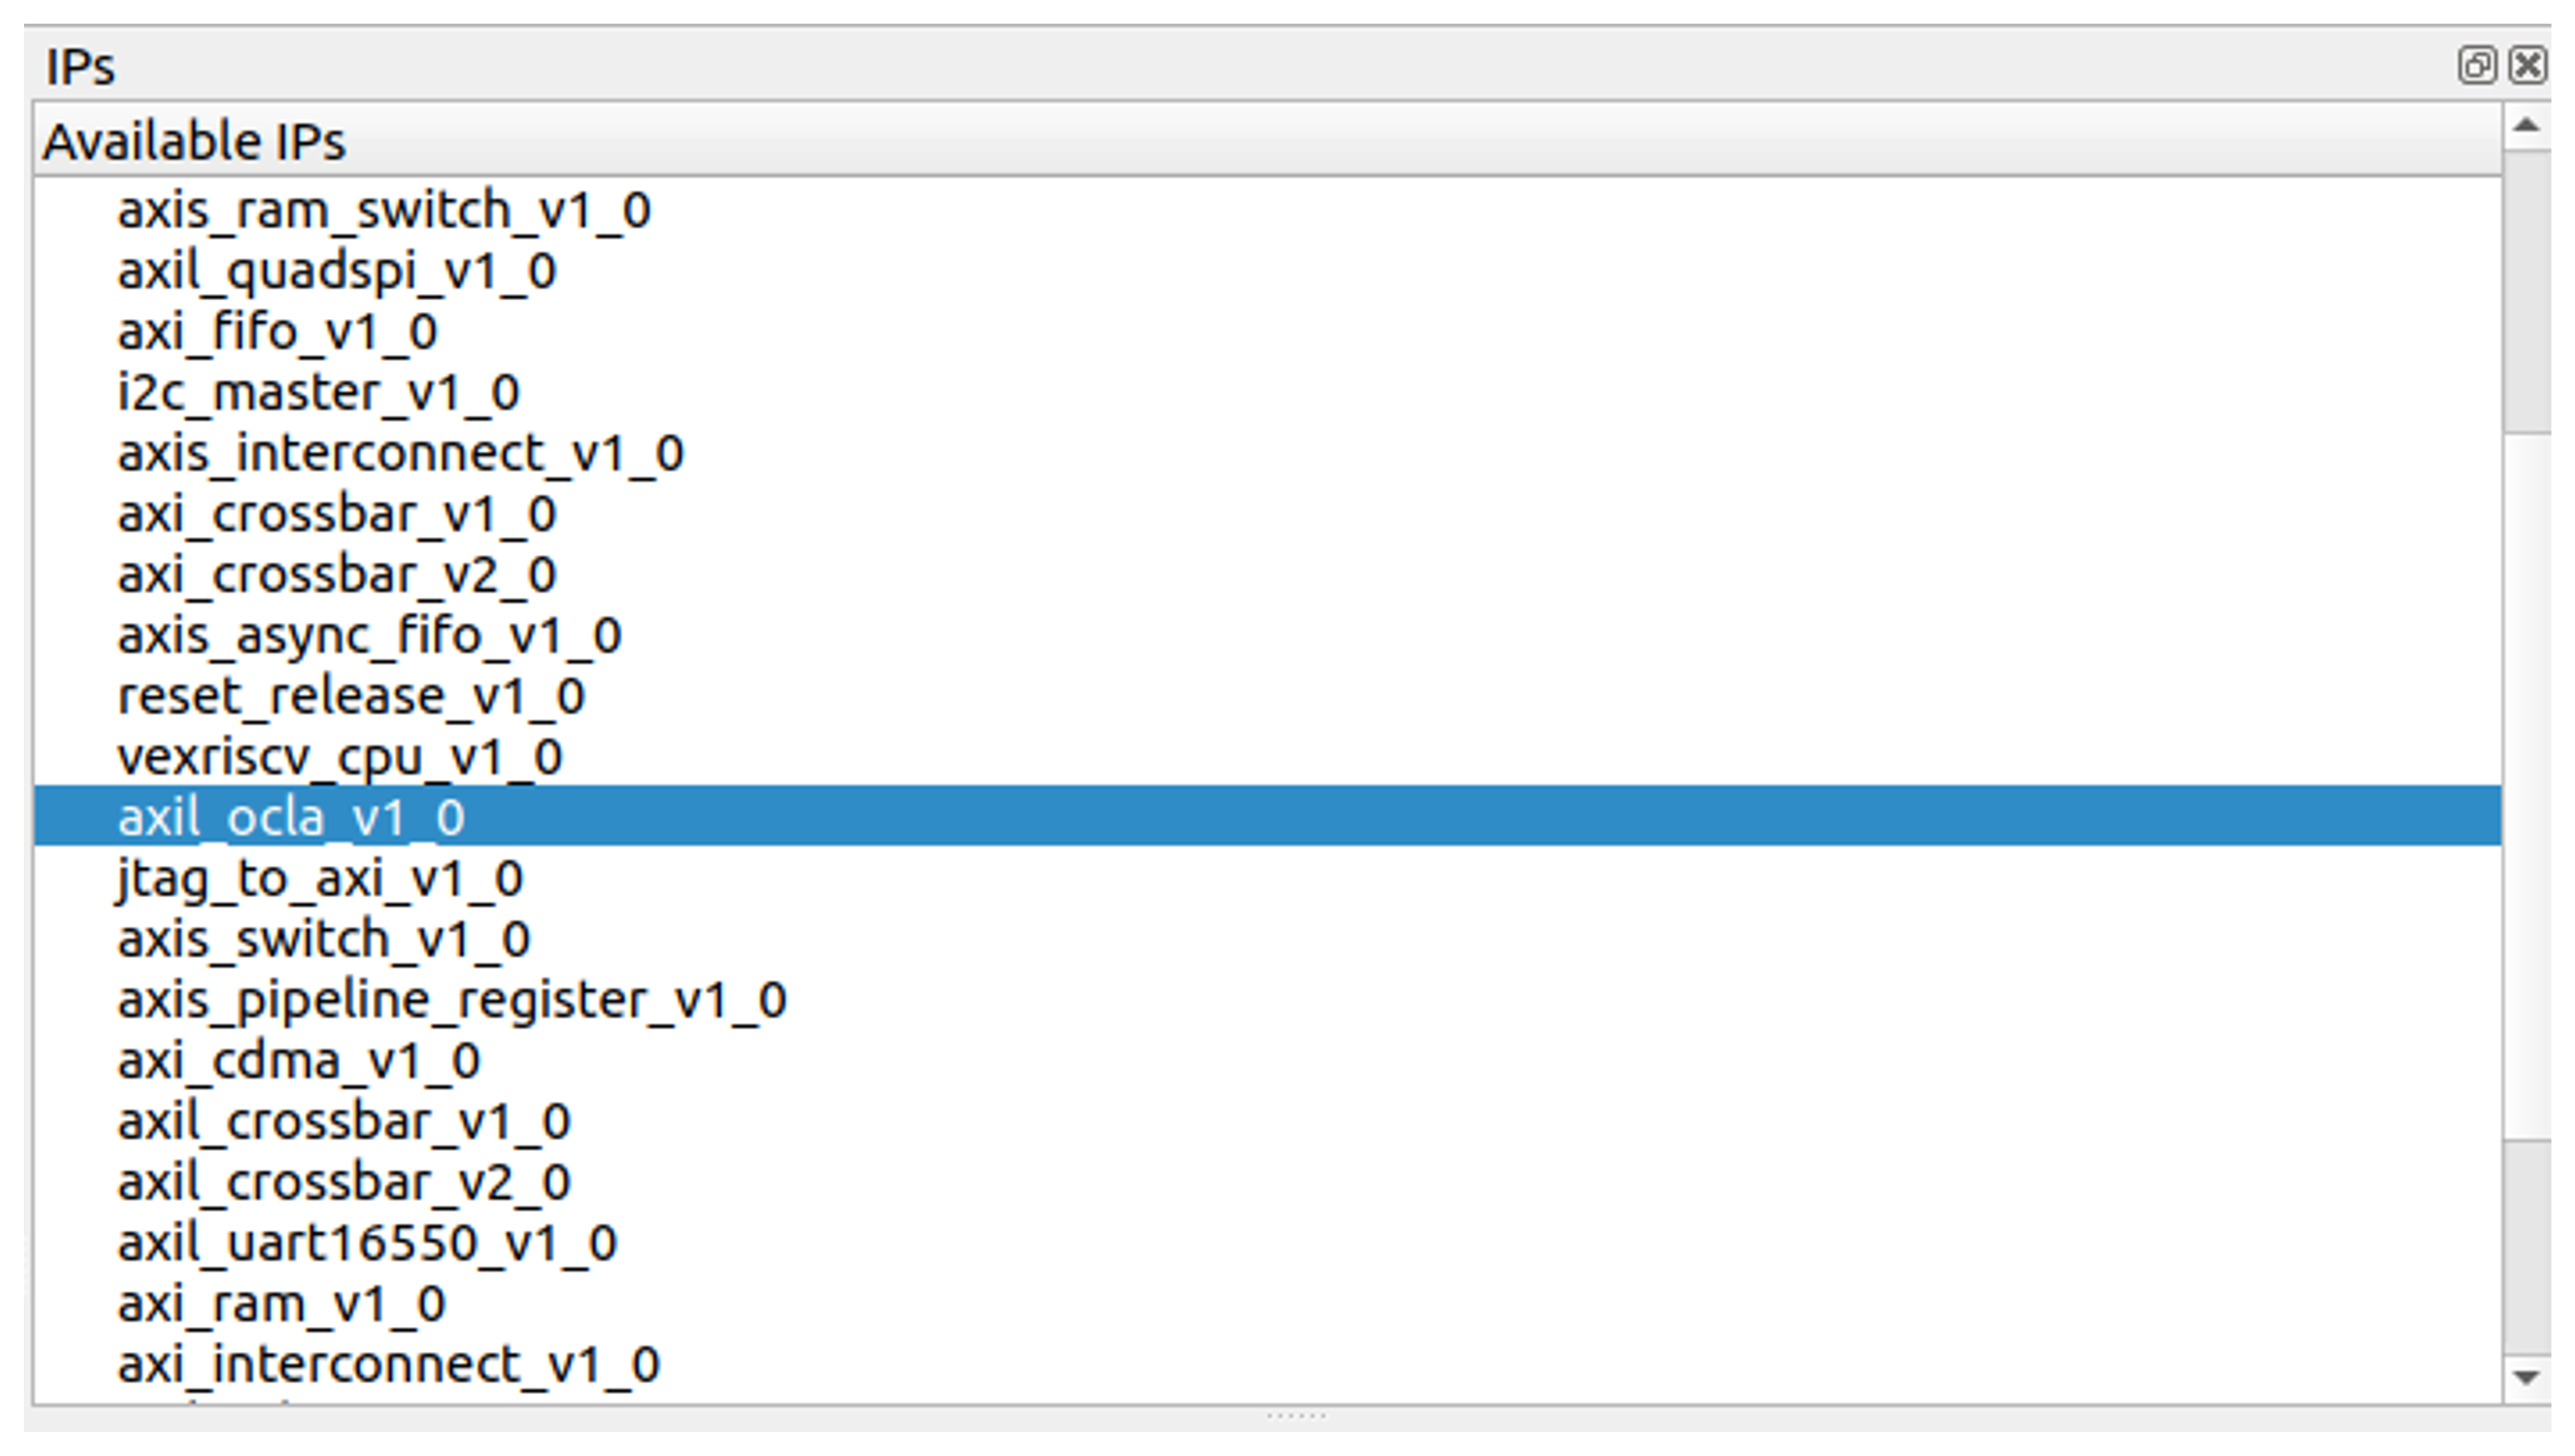
\includegraphics[width=\linewidth]{ip_1}
	\caption{\textbf{Figure \ref{fig:ip_1}.} IP list}
	\label{fig:ip_1}
\end{figure}
% \lipsum
\newpage
\paragraph{Parameters Customization:}
\addcontentsline{toc}{paragraph}{Parameters Customization}
From the IP configuration window, the parameters of the OCLA can be configured and OCLA features can be enabled for generating a customized OCLA IP core that suits the user application requirment.
\begin{figure}[h]\centering % Using \begin{figure*} makes the figure take up the entire width of the page
	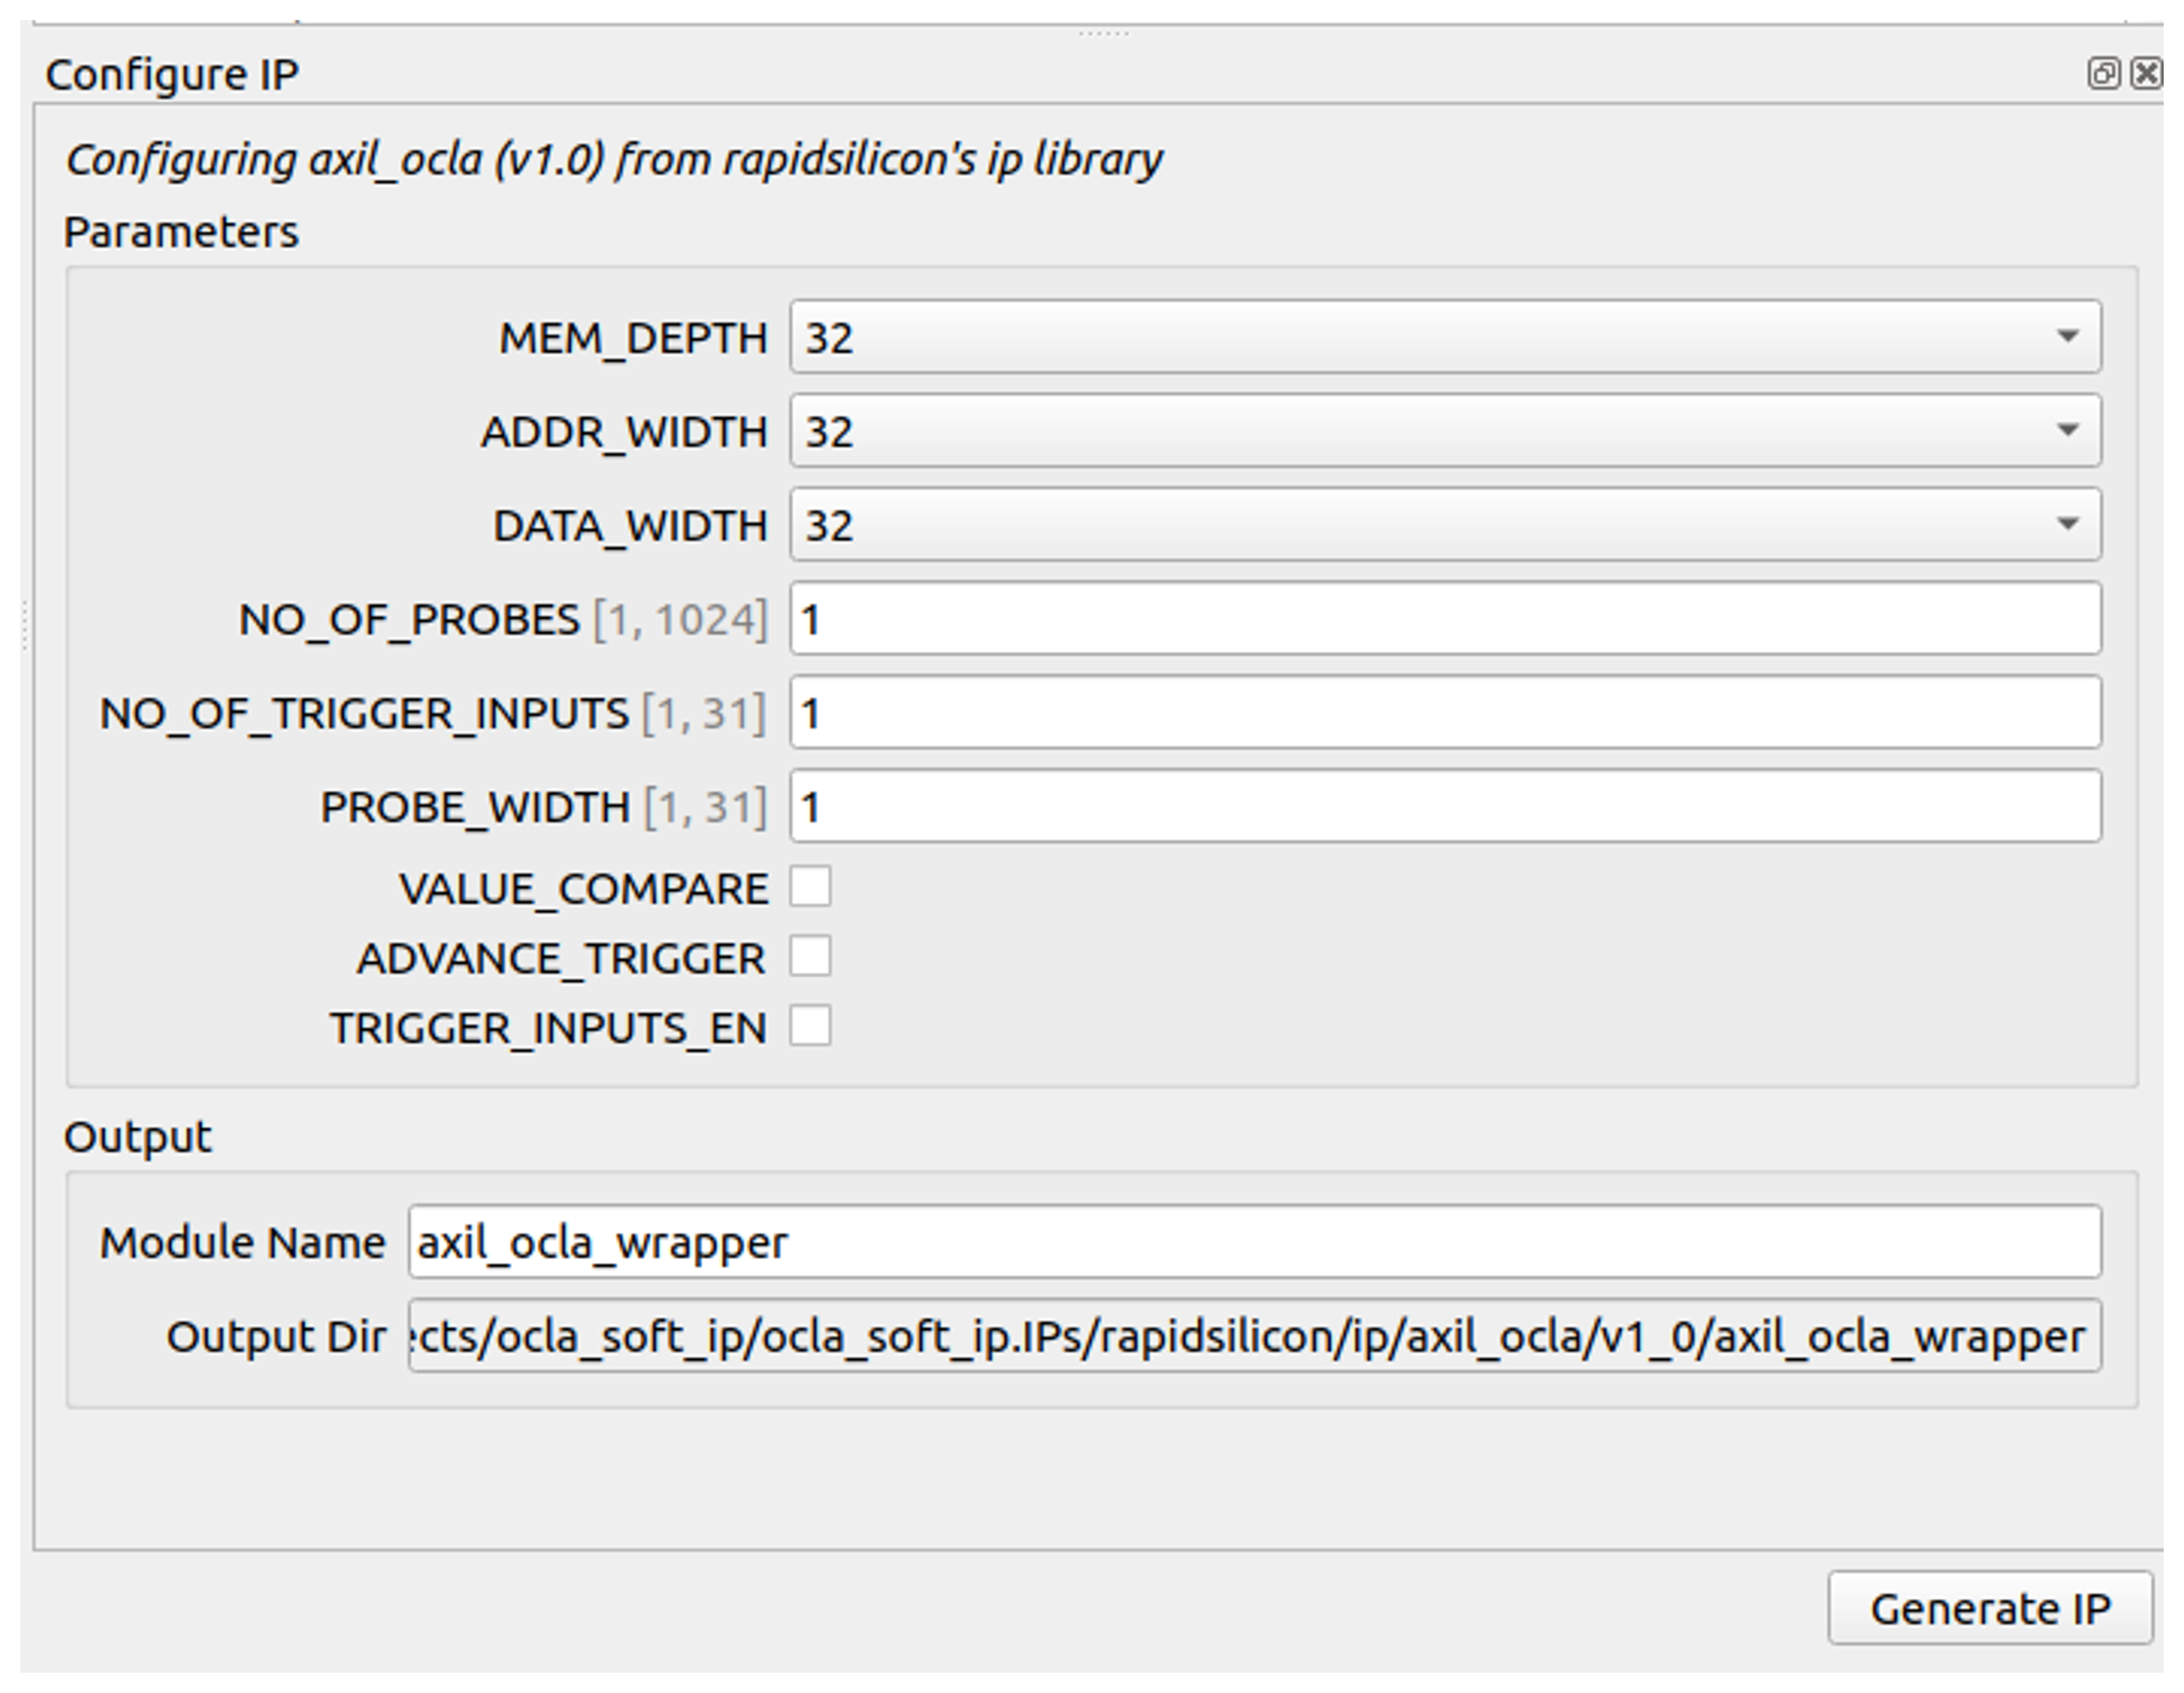
\includegraphics[width=\linewidth]{ip_2}
	\caption{\textbf{Figure \ref{fig:ip_2}.} IP Configuration }
	\label{fig:ip_2}
\end{figure}

% \lipsum


% \lipsum
